\section{PHÂN TÍCH HỆ THỐNG}

% =========================================================================
\subsection{Kiến trúc tổng thể}
Hệ thống được thiết kế gồm 3 tầng xử lý phân cấp nhằm tối ưu hóa độ trễ, khả năng chịu lỗi và tính tự chủ công nghệ:
\begin{enumerate}
    \item \textbf{Tầng Thiết bị Biên (Edge Layer - YoloUNO):} Trực tiếp đọc tín hiệu tương tự từ cảm biến khói MQ-2, tín hiệu số từ cảm biến ngọn lửa và cảm biến nhiệt/ẩm DHT11. Tầng này chịu trách nhiệm suy luận mô hình AI TinyML tại chỗ và điều khiển phản xạ cơ cấu chấp hành khẩn cấp (Servo, còi, đèn, màn hình TFT màu).
    \item \textbf{Tầng Cổng Cục Bộ (Gateway Layer - Local PC):} Đóng vai trò là trạm điều hành SCADA tại chỗ. Nhận dữ liệu telemetry qua UART Serial 115,200 baud hoặc nhận tín hiệu từ BLE (Bluetooth Low Energy), thực thi mô hình Machine Learning Isolation Forest để phát hiện các dị thường đa biến phức tạp, lưu đệm toàn bộ dữ liệu vào CSDL SQLite WAL, và cung cấp giao diện Web Monitor cục bộ tại cổng 5050.
    \item \textbf{Tầng Nền tảng Đám mây (Cloud Layer - ThingsBoard Local):} Đóng vai trò trung tâm lưu trữ lịch sử dài hạn và điều phối tự động hóa quy mô lớn thông qua RuleChain, cung cấp Dashboard công nghiệp 10 widget, bảng thông báo Notification khẩn cấp thời gian thực và quản lý lệnh RPC từ xa.
\end{enumerate}

\begin{figure}[H]
\centering
\resizebox{\textwidth}{!}{%
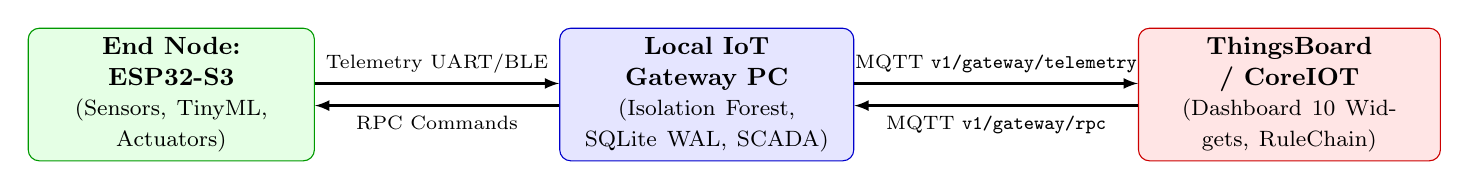
\begin{tikzpicture}[>=latex]
    \tikzset{
        block/.style={draw=blue!80!black, fill=blue!10, rectangle, rounded corners, minimum height=1.5cm, text width=3.5cm, align=center, font=\small\bfseries},
        cloud/.style={draw=red!80!black, fill=red!10, rectangle, rounded corners, minimum height=1.5cm, text width=3.6cm, align=center, font=\small\bfseries},
        edge/.style={draw=green!60!black, fill=green!10, rectangle, rounded corners, minimum height=1.5cm, text width=3.4cm, align=center, font=\small\bfseries},
        line/.style={draw, thick, ->}
    }
    
    \node [edge] (esp) at (0,0) {End Node: ESP32-S3\\{\footnotesize\normalfont (Sensors, TinyML, Actuators)}};
    \node [block] (gw) at (6.8,0) {Local IoT Gateway PC\\{\footnotesize\normalfont (Isolation Forest, SQLite WAL, SCADA)}};
    \node [cloud] (tb) at (14.2,0) {ThingsBoard / CoreIOT\\{\footnotesize\normalfont (Dashboard 10 Widgets, RuleChain)}};
    
    % Luồng dữ liệu 2 chiều ESP32 <-> Gateway
    \draw [line] ([yshift=4pt]esp.east) -- node[above, font=\scriptsize] {Telemetry UART/BLE} ([yshift=4pt]gw.west);
    \draw [line] ([yshift=-4pt]gw.west) -- node[below, font=\scriptsize] {RPC Commands} ([yshift=-4pt]esp.east);
    
    % Luồng dữ liệu 2 chiều Gateway <-> ThingsBoard
    \draw [line] ([yshift=4pt]gw.east) -- node[above, font=\scriptsize] {MQTT \texttt{v1/gateway/telemetry}} ([yshift=4pt]tb.west);
    \draw [line] ([yshift=-4pt]tb.west) -- node[below, font=\scriptsize] {MQTT \texttt{v1/gateway/rpc}} ([yshift=-4pt]gw.east);
\end{tikzpicture}%
}
\vspace{6pt}
\setlength{\abovecaptionskip}{8pt}
\caption{Sơ đồ kiến trúc luồng dữ liệu hai chiều của hệ thống}
\label{fig:sodo_kientruc}
\end{figure}

\subsection{Phân rã chức năng}
Hệ thống được phân rã thành 5 khối chức năng chính hoạt động phối hợp đồng bộ:
\begin{itemize}
    \item \textbf{Khối thu thập dữ liệu \& tiền xử lý:} Chuyển đổi tín hiệu ADC 12-bit, chuẩn hóa Z-Score, loại trừ nhiễu cảm biến trong 5 giây khởi động đầu tiên (Warmup Phase).
    \item \textbf{Khối suy luận AI nhị phân (Edge TinyML):} Tính toán xác suất nguy cơ cháy từ vectơ đặc trưng [Khói, Lửa, Nhiệt, Ẩm], nội suy tức thời $<0.1\text{ ms}$.
    \item \textbf{Khối phát hiện dị thường (Fog Isolation Forest):} Đánh giá độ lệch chuẩn đa biến, phát hiện bất thường môi trường bất kể ngưỡng cố định.
    \item \textbf{Khối đệm ngoại tuyến (Store-and-Forward):} Ghi dữ liệu đồng thời vào RAM và SQLite WAL, tự động phát hiện mất mạng để đệm offline và đồng bộ bù khi có kết nối trở lại.
    \item \textbf{Khối giám sát \& điều khiển hai chiều (SCADA \& RPC):} Điều khiển tức thì cơ cấu Servo đóng/mở cửa thoát hiểm, còi hú và đèn chớp từ Web cục bộ hoặc ThingsBoard.
\end{itemize}
% =========================================================================
\subsection{Phân lớp tính năng}
\subsubsection{Lớp cảm biến}
\begin{itemize}
    \item \textbf{Cảm biến khí gas/khói MQ-2:} Đọc qua kênh ADC 12-bit (GPIO 1), tầm đo $0 - 4095\text{ ADC}$. Không khí sạch đạt $140 - 220\text{ ADC}$, ngưỡng khói cảnh báo $800\text{ ADC}$, ngưỡng cháy $1800\text{ ADC}$.
    \item \textbf{Cảm biến ngọn lửa bước sóng hồng ngoại:} Đọc qua kênh số GPIO 2. Bình thường ngõ ra mức 1, khi có lửa phát xạ bước sóng $760 - 1100\text{ nm}$ ngõ ra kéo về mức 0 (Active LOW).
    \item \textbf{Cảm biến nhiệt độ và độ ẩm DHT11:} Đọc qua giao tiếp 1-Wire tại GPIO 4, chu kỳ lấy mẫu 1 giây, độ phân giải $1^\circ\text{C}$ và $1\% RH$.
\end{itemize}
% =========================================================================
\subsubsection{Lớp giao tiếp}
\begin{itemize}
    \item \textbf{Giao tiếp vi điều khiển -- Gateway qua UART/BLE (T08):} Tốc độ baud 115,200 bps, định dạng khung bản tin văn bản và chuỗi JSON thu gọn.
    \item \textbf{Giao tiếp không dây Bluetooth Low Energy (T03):} Vi điều khiển ESP32-S3 khởi tạo GATT Server với tên \texttt{YoloUNO\_FireNode}. Cung cấp Telemetry Characteristic (Notify) để đẩy dữ liệu không dây và Command Characteristic (Write) để nhận lệnh điều khiển trực tiếp từ Gateway qua thư viện \texttt{bleak}.
    \item \textbf{Giao tiếp Gateway -- ThingsBoard (MQTT Gateway API - T15):} Sử dụng bộ topic chuẩn của ThingsBoard IoT Gateway:
    \texttt{v1/gateway/connect}, \texttt{v1/gateway/telemetry}, và \texttt{v1/gateway/rpc}.
\end{itemize}
% =========================================================================
\subsubsection{Lớp IoT Gateway}
Hiện thực trên môi trường Python với kiến trúc đa luồng: Luồng chính đọc Serial/BLE, luồng HTTP hosting giao diện Keen SCADA tại cổng 5050, luồng Command Worker dispatch lệnh điều khiển phi khóa (non-blocking), và luồng Sync Worker quản lý đệm CSDL SQLite WAL.
% =========================================================================
\subsubsection{Lớp trí tuệ nhân tạo (Dual-AI)}
\begin{itemize}
    \item \textbf{Edge TinyML (ESP32-S3):} Bộ phân loại hồi quy Logistic tối ưu hóa với hàm kích hoạt Sigmoid, tính toán hoàn toàn bằng số học dấu phẩy động 32-bit trên nhân Tensilica Xtensa LX7 kép 240MHz.
    \item \textbf{Fog AI (Gateway PC):} Thuật toán cây ngẫu nhiên Isolation Forest với tham số $contamination=0.08$, tự động cập nhật cửa sổ trượt (sliding window 60 mẫu).
\end{itemize}
% =========================================================================
\subsubsection{Lớp ứng dụng và nền tảng CoreIOT}
Triển khai phiên bản ThingsBoard trên Docker Localhost (cổng 9090 và 1883). Thiết kế Dashboard công nghiệp 10 widget trực quan. Xây dựng RuleChain phân loại 3 cấp độ tự động tạo/xóa Alarm và bắn thông báo Notification thời gian thực lên Dashboard. Đồng thời tích hợp cơ chế cập nhật firmware từ xa qua mạng vô tuyến OTA (Over-The-Air - T14) quản lý phiên bản phần mềm tự động không cần cắm nạp cáp vật lý.
% =========================================================================
\subsection{Ánh xạ tính năng -- yếu tố công nghệ}
Bảng~\ref{tab:anh_xa_cong_nghe} thể hiện sự đối chiếu tường minh giữa tính năng hệ thống và danh mục tiêu chí đánh giá BTL của giảng viên.

\begin{table}[H]
\centering
\small
\setlength{\tabcolsep}{4pt}
\renewcommand{\arraystretch}{1.25}
\caption{Bảng ánh xạ tính năng hệ thống vào các tiêu chí công nghệ BTL}
\label{tab:anh_xa_cong_nghe}
\begin{tabularx}{\textwidth}{|>{\raggedright\arraybackslash}X|>{\centering\arraybackslash}p{1.9cm}|>{\centering\arraybackslash}p{2.4cm}|}
\hline
\textbf{Mô Tả Tính Năng} & \textbf{Mã Tiêu Chí} & \textbf{Điểm Quy Định} \\ \hline
Truyền thông không dây BLE năng lượng thấp giữa cảm biến và Gateway & T03 & 1.5 \\ \hline
Thu thập cảm biến, hiển thị TFT và kích hoạt cơ cấu chấp hành & T04, T10 & 1.0 + 1.0 \\ \hline
Suy luận mô hình học máy TinyML trực tiếp trên vi điều khiển & T04 & 1.0 \\ \hline
Công cụ huấn luyện tự động, chuẩn hóa dữ liệu và xuất mã C & T05 & 1.0 \\ \hline
IoT Gateway PC giao tiếp UART hai chiều và đẩy MQTT lên Cloud & T08 & 1.0 \\ \hline
Thuật toán Isolation Forest phát hiện dị thường trên Gateway & T09 & 1.0 \\ \hline
Giao diện SCADA Web Monitor 5050 lưu vết sự kiện thời gian thực & T10, N06 & 1.0 + 1.0 \\ \hline
Cơ chế đồng bộ Store-and-Forward đệm ngoại tuyến SQLite WAL & T15 & 2.0 \\ \hline
Dashboard ThingsBoard 10 widget, RuleChain 3 cấp độ, Web Notification & T11, T12, T13 & 1.0 + 1.0 + 0.5 \\ \hline
Cập nhật firmware qua OTA không dây qua Wi-Fi / ThingsBoard OTA & T14 & 2.0 \\ \hline
Tự triển khai máy chủ ThingsBoard CE cục bộ bằng Docker Desktop & N07 & 1.0 \\ \hline
\end{tabularx}
\end{table}
% =========================================================================
\subsection{Danh sách thiết bị phần cứng}
\begin{table}[H]
\centering
\caption{Danh mục linh kiện phần cứng sử dụng trong đề tài}
\label{tab:linh_kien}
\begin{tabular}{|c|l|c|p{5.5cm}|}
\hline
\textbf{STT} & \textbf{Tên linh kiện} & \textbf{Số lượng} & \textbf{Thông số kỹ thuật / Chức năng} \\ \hline
1 & ESP32-S3 YoloUNO & 1 & Dual-Core Xtensa LX7 240MHz, 512KB SRAM, 8MB Flash \\ \hline
2 & Màn hình màu TFT LCD 2.4" & 1 & Độ phân giải 320x240, driver ST7789 qua giao tiếp SPI \\ \hline
3 & Cảm biến khói/gas MQ-2 & 1 & Đo nồng độ LPG, Propane, Methane, Khói; ngõ ra Analog ADC \\ \hline
4 & Cảm biến ngọn lửa hồng ngoại & 1 & Bước sóng nhận diện 760nm -- 1100nm, góc quét $60^\circ$ \\ \hline
5 & Cảm biến nhiệt ẩm DHT11 & 1 & Dải nhiệt $0 - 50^\circ\text{C}$, dải ẩm $20 - 90\% RH$ \\ \hline
6 & Động cơ Servo TowerPro SG90 & 1 & Góc xoay $0^\circ - 180^\circ$, điều khiển cửa thoát hiểm \\ \hline
7 & Còi báo động Active Buzzer 5V & 1 & Âm lượng $>85\text{ dB}$, báo động âm thanh cục bộ \\ \hline
8 & Đèn LED cảnh báo đỏ 5mm & 1 & Cảnh báo thị giác tại chỗ \\ \hline
\end{tabular}
\end{table}
\newpage

